\documentclass[a4paper,UTF8]{article}
\usepackage{ctex}
\usepackage[margin=1.25in]{geometry}
\usepackage{color}
\usepackage{graphicx}
\usepackage{amssymb}
\usepackage{amsmath}
\usepackage{amsthm}
\usepackage{soul, color, xcolor}
\usepackage{bm}
\usepackage{tcolorbox}
\usepackage{hyperref}
\numberwithin{equation}{section}
%\usepackage[thmmarks, amsmath, thref]{ntheorem}
\theoremstyle{definition}
\newtheorem*{solution}{Solution}
\newtheorem*{prove}{Proof}
\usepackage{multirow}
\usepackage{diagbox}
\usepackage{float}

\def \X {\boldsymbol{X}}
\def \Y {\boldsymbol{Y}}
\def \A {\boldsymbol{A}}
\def \w {\boldsymbol{w}}
\def \u {\boldsymbol{u}}
\def \v {\boldsymbol{v}}
\def \s {\boldsymbol{s}}
\def \y {\boldsymbol{y}}
\def \x {\boldsymbol{x}}
\def \z {\boldsymbol{z}}
\def \hy {\widehat{y}}
\def \by {\Bar{y}}
\def \H {\mathbf{H}}
\def \I {\mathbf{I}}
\def \boldalpha {\boldsymbol{\alpha}}
\newcommand\given[1][]{\:#1\vert\:}
\setlength{\parindent}{0pt}
%--

%--
\begin{document}
\title{机器学习导论\ 习题三}
\author{211300063, 张运吉, \href{mailto:邮箱}{211300063@smail.nju.edu.cn}}
\maketitle
\section*{作业提交注意事项}
\begin{tcolorbox}
	\begin{enumerate}
		\item[1.] 请在LaTeX模板中第一页填写个人的学号、姓名、邮箱;
		\item[2.] 本次作业需提交作答后的该 pdf 文件、编程题代码(.py文件); {\color{red}\textbf{请将二者打包为~.zip 文件上传}}. 注意命名规则, 三个文件均命名为 “$\text{学号}\_\text{姓名}$” + “$.\text{后缀}$” (例如“$\text{211300001}\_\text{张三}$” + “.pdf”、“.py”、“.zip”);
		\item[3.] 若多次提交作业, 则在命名~.zip 文件时加上版本号, 例如“211300001\_张三\_v1.zip” (批改时以版本号最高的文件为准);
		\item[4.] 本次作业提交截止时间为 {\color{red}\textbf{ 5 月 2 日23:59:59}}. 未按照要求提交作业, 提交作业格式不正确, {\color{red}\textbf{作业命名不规范}}, 将会被扣除部分作业分数; 除特殊原因 (如因病缓交, 需出示医院假条) 逾期未交作业, 本次作业记 0 分; {\color{red}\textbf{如发现抄袭, 抄袭和被抄袭双方成绩全部取消}};
		\item[5.] 本次作业提交地址为 \href{https://box.nju.edu.cn/u/d/71102ced9a9b4d6f8d05/}{here}, 请大家预留时间提前上交, 以防在临近截止日期时, 因网络等原因无法按时提交作业.
	\end{enumerate}
\end{tcolorbox}
\newpage

\section{[20pts] Representor Theorem}
表示定理告诉我们, 对于一般的损失函数和正则化项,优化问题的最优解都可以表示为核函数的线性组合. 我们将尝试证明表示定理的简化版本, 
并在一个实际例子中对其进行应用. 请仔细阅读《机器学习》第六章6.6节, 并回答如下问题.
\begin{enumerate}
    \item[(1)] \textbf{[10pts]} 考虑通过引入核函数来将线性学习器拓展为非线性学习器, 优化目标由结构风险和经验风险组成:
    \begin{align*}
        \min_{\w} \  J(\w) = \frac{1}{N} \sum_{i=1}^N \mathcal{L}\left(\w^T \phi(\x_i), y_i \right) + \frac{\lambda}{2}\|\w\|^2,
    \end{align*}
    其中映射$\phi: \mathcal{X} \to \mathbb{H}$将样本映射到特征空间$\mathbb{H}$, $\mathcal{L}$为常见的损失函数,
    并记$\X = \left[\phi(\x_1), \cdots, \phi(\x_m)\right]$为映射后的数据矩阵. 请证明: 优化问题的最优解$\w^\star$属于矩阵$\X$的列空间, 即$\w^\star \in \mathcal{C}(\X)$.

    (提示: 给定线性子空间$\mathcal{S}$, 任意向量$\u$有唯一的正交分解$\u = \v + \s(\v \in \mathcal{S}, \s \in \mathcal{S}^{\perp})$. 你需要选取合适的线性子空间, 对$\w$进行正交分解)
    \item[(2)] \textbf{[10pts]} 在核岭回归问题(KRR, kernel ridge regression)中, 优化目标为:
    \begin{align*}
        \min_{\w} \  F(\w) = \lambda\|\w\|^2+\sum_{i=1}^m\left(\w^T\phi(\x_i)-y_i\right)^2.
    \end{align*}
    根据第一问的结论, 该优化问题的最优解满足$\w_{\text{KRR}}^\star = \X \boldalpha$. 请给出此处$\boldalpha$的具体形式. 值得一提的是, $\boldalpha$
    是KRR问题对偶问题的最优解.

    (提示: 你需要先求出$\w_{\text{KRR}}^\star$的具体形式)
\end{enumerate}

\begin{solution}
	此处用于写解答(中英文均可)
	~\\
	~\\
	~\\
    \begin{enumerate}
        \item [(1)]
        $\mathcal{S} = \mathcal{C}(\X) = \operatorname{span}\left(\phi\left(\boldsymbol{x}_{1}\right), \ldots, \phi\left(\boldsymbol{x}_{m}\right)\right)$是特征空间$\mathbb{H}$的线性子空间\\
        则对任意向量$\w$有唯一的正交分解$\w = \v + \s(\v \in \mathcal{S}, \s \in \mathcal{S}^{\perp})$. \\
        \begin{equation}
            \boldsymbol{s}^{T} \phi\left(\boldsymbol{x}_{i}\right) = 0 \text{ due to }  \phi\left(\boldsymbol{x}_{i}\right) \in \mathcal{S}, \s \in \mathcal{S}^{\perp}
        \end{equation}
        由此可得:
        \begin{equation}
            \begin{aligned} J(\boldsymbol{w}) & =\frac{1}{N} \sum_{i=1}^{N} \mathcal{L}\left(\boldsymbol{v}^{T} \phi\left(\boldsymbol{x}_{i}\right)+\boldsymbol{s}^{T} \phi\left(\boldsymbol{x}_{i}\right), y_{i}\right)+\frac{\lambda}{2}\|\boldsymbol{w}\|^{2} \\ & =\frac{1}{N} \sum_{i=1}^{N} \mathcal{L}\left(\boldsymbol{v}^{T} \phi\left(\boldsymbol{x}_{i}\right), y_{i}\right)+\frac{\lambda}{2}\|\boldsymbol{w}\|^{2}\end{aligned} \label{J}
        \end{equation}
        设$\w^{\star}=\v^{\star}+\s^{\star}$,根据最优条件:$J(\w^{\star}) \leq J(\v^{\star})$ \\
        代入公式\ref*{J}得:
        \begin{equation}
            \begin{array}{c}\left\|\v^{\star}+\s^{\star}\right\|^{2} \leq\left\|\v^{\star}\right\|^{2} \\ \v^{\star \top} \v^{\star}+\s^{\star \top} \s^{\star} \leq \v^{\star \top} \v^{\star}\end{array}
        \end{equation}
        所以:$\s = \bold{0}$, $\w^{\star}=\v^{\star} \in \mathcal{S}= \mathcal{C}(\X)$\\
        说明:优化问题的最优解$\w^\star$属于矩阵$\X$的列空间
        \item [(2)]
        优化函数$F(\w)$是关于$\w$的凸函数,所以令$F(\w)$的导数等于0即可求得最优解$\w_{\text{KRR}}^\star$.\\
        \begin{equation}
            \begin{aligned} \nabla F(\boldsymbol{w}) & =2 \lambda \boldsymbol{w}+2 \sum_{i=1}^{m} \phi\left(\boldsymbol{x}_{i}\right)\left(\phi\left(\boldsymbol{x}_{i}\right)^{\top} \boldsymbol{w}-y_{i}\right) \\ &= 2\lambda\mathbf{I}\boldsymbol{w}+2(\boldsymbol{X}\boldsymbol{X}^{\top}\boldsymbol{w}-\boldsymbol{X}y)\\& =-2 \boldsymbol{X} \boldsymbol{y}+2\left(\boldsymbol{X} \boldsymbol{X}^{\top}+\lambda \mathbf{I}\right) \boldsymbol{w}=0\end{aligned}
        \end{equation}
        解得:$$\boldsymbol{w}_{\mathrm{KRR}}^{\star}=\left(\boldsymbol{X} \boldsymbol{X}^{\top}+\lambda \mathbf{I}\right)^{-1} \boldsymbol{X} \boldsymbol{y}=\boldsymbol{X}\left(\lambda \mathbf{I}+\boldsymbol{X}^{\top} \boldsymbol{X}\right)^{-1} \boldsymbol{y}$$
        所以: $$\alpha = \left(\lambda \mathbf{I}+\boldsymbol{X}^{\top} \boldsymbol{X}\right)^{-1} \boldsymbol{y}$$
    \end{enumerate}
\end{solution}

\newpage

\section{[20pts] Leave-One-Out error in SVM}
《机器学习》第2.2.2节中我们接触到了留一法(Leave-One-Out), 使用留一损失作为分类器泛化错误率的估计, 即: 每次将一个样本作为测试集, 其余样本作为训练集, 最后对所有的测试误差取平均. 对于SVM算法$\mathcal{A}$, 令$h_{S}$为该算法在训练集$S$上的输出, 则$\mathcal{A}$的经验留一损失可形式化为
\begin{align*}
    \hat R_{\text{LOO}}(\mathcal{A}) = \frac1m \sum_{i=1}^m \mathrm{1}_{h_{S \setminus \{\x_i\}}(\x_i) \neq y_i}.
\end{align*}
本题将通过探索留一损失的一些数学性质, 分析SVM泛化误差与支持向量个数的联系, 并给出一个期望意义下的泛化误差界. (注: 本题仅考虑可分情形, 即数据集是线性可分的)
\begin{enumerate}
	\item[(1)] \textbf{[5pts]} 在实际应用中, 测试误差相比于泛化误差是很容易获取的. 我们往往希望测试误差是泛化误差较为准确的估计, 至少应该是无偏估计. 试证明留一损失是数据集大小为$m-1$时泛化误差的无偏估计, 即
	\begin{align*}
        \mathbb{E}_{S \sim \mathcal{D}^m}[\hat{R}_{\mathrm{LOO}}(\mathcal{A})]=\mathbb{E}_{S^{\prime} \sim \mathcal{D}^{m-1}}\left[R\left(h_{S^{\prime}}\right)\right].
    \end{align*}
	\item[(2)] \textbf{[5pts]} SVM的最终模型仅与支持向量有关, 支持向量完全刻画了决策边界. 这一现象可以抽象表示为, 如果样本$\x$并非$h_S$的支持向量, 则移除该样本不会改变SVM模型, 即$h_{S \setminus \{\x\}} = h_S$. 这一性质在分析误差时有关键作用, 考虑如下问题:
	如果$\x$不是$h_S$的支持向量, $h_{S \setminus \{\x\}}$会将$x$正确分类吗, 为什么? 该问题的结论的逆否命题是什么? 
	\item[(3)] \textbf{[10pts]} 基于上一小问的结果, 试证明下述SVM的泛化误差界限:
	\begin{align*}
        \mathbb{E}_{S \sim \mathcal{D}^m}\left[R(h_S)\right] \leq \mathbb{E}_{S \sim \mathcal{D}^{m+1}} \left[\frac{N_{SV}(S)}{m+1}\right],
    \end{align*}
    其中$N_{SV}(S)$为模型$h_S$支持向量的个数. 从这一泛化误差界中, 我们能够看到SVM的泛化能力与支持向量个数之间有紧密的联系.

\end{enumerate}

\begin{solution}
	此处用于写解答(中英文均可)
	~\\
	~\\
	~\\
    \begin{enumerate}
        \item [(1)]
        证明:
        \begin{equation}
            \begin{aligned} \mathbb{E}_{S \sim D^{m}}[\hat{R}_{\mathrm{LOO}}(\mathcal{A})] & =\frac{1}{m} \sum_{i=1}^{m} \mathbb{E}_{S \sim D^{m}}\left[1_{h_{S-\left\{x_{i}\right\}}\left(x_{i}\right) \neq y_{i}}\right] \\ & =\mathbb{E}_{S \sim D ^m}\left[1_{h_{S-\left\{x_{1}\right\}}\left(x_{1}\right) \neq y_{1}}\right] \\ & =\mathbb{E}_{S^{\prime} \sim D^{m-1}, x_{1} \sim D}\left[1_{h_{S^{\prime}}\left(x_{1}\right) \neq y_{1}}\right] \\ & =\mathbb{E}_{S^{\prime} \sim D^{m-1}}\left[\mathbb{E}_{x_{1} \sim D}\left[1_{h_{S^{\prime}}\left(x_{1}\right) \neq y_{1}}\right]\right] \\ & =\mathbb{E}_{S^{\prime} \sim D^{m-1}}\left[R\left(h_{S^{\prime}}\right)\right] \end{aligned} \label{2}
        \end{equation}
        \item [(2)]
        可以.\\
        根据支持向量机得定义,如果样本$\x$并非$h_S$的支持向量,那么$yh_S>1$($y$是样本$\x$的ground true),因为$h_{S \setminus \{\x\}} = h_S$,
        所以$yh_{S \setminus \{\x\}} > 1$, 说明$h_{S \setminus \{\x\}}$可以将$x$正确分类. \\
        逆否命题:如果$h_{S \setminus \{\x\}}$ 不能将$\x$正确分类,那么$\x$是 $h_S$的支持向量.
        \item [(3)]
        假设$S$是一个线性可分的样本,样本个数为$m+1$. \\
        根据(2)的结论,如果$h_{S \setminus \{\x\}}$ 不能将$\x$正确分类,那么$\x$是 $h_S$的支持向量.\\
        所以留一法中分类错误的样本个数小于等于$h_S$的支持向量个数. \\
        \begin{equation}
            \begin{aligned}
                \hat R_{\text{LOO}}(\mathcal{A}) &= \frac{1}{m+1} \sum_{i=1}^{m+1} \mathrm{1}_{h_{S \setminus \{\x_i\}}(\x_i) \neq y_i} \\
                & \leq \frac{1}{m+1}N_{SV}(S)
            \end{aligned}
        \end{equation}
        两边取期望:
        $$\mathbb{E}_{S \sim D^{m+1}}[\hat R_{\text{LOO}}(\mathcal{A})] \leq \mathbb{E}_{S \sim \mathcal{D}^{m+1}} \left[\frac{N_{SV}(S)}{m+1}\right] $$
        再由(1)的结论可知:
        \begin{align*}
            \mathbb{E}_{S \sim \mathcal{D}^m}\left[R(h_S)\right] \leq \mathbb{E}_{S \sim \mathcal{D}^{m+1}} \left[\frac{N_{SV}(S)}{m+1}\right]
        \end{align*}
    \end{enumerate}
\end{solution}

\newpage

\section{[30pts] Margin Distribution}
SVM的核心思想是最大化最小间隔, 以获得最鲁棒的分类决策边界. 然而, 近年来的一些理论研究表明, 最大化最小间隔并不一定会带来更好的泛化能力,
反而优化样本间隔的分布可以更好地提高泛化性能. 为了刻画间隔的分布, 我们可以使用样本间隔的一阶信息和二阶信息, 即间隔均值和间隔方差. 

给定训练数据集$\mathcal{S} = \{(\x_1, y_1), \cdots, (\x_m, y_m)\}$, $\phi: \mathcal{X} \to \mathbb{H}$为映射函数, 
我们记$\X = \left[\phi(\x_1), \cdots, \phi(\x_m)\right]$为映射后的数据矩阵, $\y^T = [y_1, \cdots, y_m]$为标签向量, $\Y$是对角元素为$y_1, \cdots, y_m$的对角矩阵. 请回答如下问题.
\begin{enumerate}
    \item[(1)] \textbf{[5pts]} 间隔均值与间隔方差分别定义为:
    \begin{align*}
        &\gamma_m = \frac1m \sum_{i=1}^m y_i \w^T \phi(\x_i), \\
        &\gamma_v = \frac1m \sum_{i=1}^m (y_i\w^T\phi(\x_i) - \gamma_m)^2.
    \end{align*}
    请使用题给记号, 化简上述表达式.
    \item[(2)] \textbf{[5pts]} 考虑标准的软间隔SVM(课本公式(6.35))且引入核函数. 现在, 我们希望在其基础上进行改进: 最大化样本间隔的均值, 并且最小化样本间隔的方差. 令间隔均值的相对权重
    为$\mu_1$, 间隔方差的相对权重为$\mu_2$, 请给出相应的优化问题.
    \item[(3)] \textbf{[20pts]} 第二问中的想法十分直接, 但是由于优化问题中的目标函数形式较为复杂, 导致对偶问题难以表示. 借鉴SVM中固定最小间隔为1的思路, 我们固定间隔均值为$\gamma_m = 1$,
    每个样本$(\x_i, y_i)$的间隔相较于均值的偏移为$\lvert y_i \w^T \phi(\x_i) - 1\rvert$. 此时仅需最小化间隔方差, 相应的优化问题为
    \begin{align*}
        \min _{\boldsymbol{w}, \xi_i, \epsilon_i} & \quad \frac{1}{2}\|\boldsymbol{w}\|^2+ \frac{C}{m} \sum_{i=1}^m\left(\xi_i^2+\epsilon_i^2\right) \\
        \text { s.t. } & \quad y_i \boldsymbol{w}^{\top} \phi\left(\x_i\right) \geq 1-\xi_i, y_i \boldsymbol{w}^{\top} \phi\left(\x_i\right) \leq 1+\epsilon_i, \forall i .
    \end{align*}
    其中$C > 0$为正则化系数, $\xi_i$和$\epsilon_i$为松弛变量, 刻画了样本相较于均值的偏移程度. 进一步地, 我们借鉴支持向量回归(SVR)中的做法, 引入$\theta$-不敏感损失函数, 
    容忍偏移小于$\theta$的样本. 同时, 间隔均值两侧的松弛程度可有所不同, 使用参数$\mu$进行平衡. 最终我们得到了最优间隔分布机(Optimal margin Distribution Machine)的优化问题:
    \begin{align*}
        \min _{\boldsymbol{w}, \xi_i, \epsilon_i} & \quad \frac{1}{2}\|\boldsymbol{w}\|^2+ \frac{C}{m} \sum_{i=1}^m \frac{\xi_i^2+\mu \epsilon_i^2}{(1-\theta)^2} \\
        \text { s.t. } & \quad y_i \boldsymbol{w}^{\top} \phi\left(\x_i\right) \geq 1-\theta-\xi_i \\
        & \quad y_i \boldsymbol{w}^{\top} \phi\left(\x_i\right) \leq 1+\theta+\epsilon_i, \forall i.
    \end{align*}
    试推导该问题的对偶问题, 要求详细的推导步骤.
    (提示: 借助题干中的记号, 将该优化问题表达成矩阵的形式. 你也可以引入额外的记号)
\end{enumerate}

\begin{solution}
	此处用于写解答(中英文均可)
	~\\
    \begin{enumerate}
        \item [(1)]
        \begin{equation}
            \begin{aligned} \gamma_{m} & =\frac{1}{m} \sum_{i=1}^{m} y_{i} \boldsymbol{w}^{T} \phi\left(\boldsymbol{x}_{i}\right)=\frac{1}{m} \boldsymbol{w}^{\top} \boldsymbol{X} \boldsymbol{y} \\ \gamma_{v} & =\frac{1}{m} \sum_{i=1}^{m}\left(y_{i} \boldsymbol{w}^{T} \phi\left(\boldsymbol{x}_{i}\right)-\gamma_{m}\right)^{2} \\ & =\frac{1}{m} \sum_{i=1}^{m}\left(y_{i} \boldsymbol{w}^{\top} \phi\left(\boldsymbol{x}_{i}\right) y_{i} \boldsymbol{w}^{\top} \phi\left(\boldsymbol{x}_{i}\right)-2 y_{i} \boldsymbol{w}^{\top} \phi\left(\boldsymbol{x}_{i}\right) \gamma_{m}+\gamma_{m}^{2}\right) \\ & =\frac{1}{m}\left[\sum_{i=1}^{m}\left(y_{i}^2 \boldsymbol{w}^{\top} \phi\left(\boldsymbol{x}_{i}\right) \boldsymbol{w}^{\top} \phi\left(\boldsymbol{x}_{i}\right)\right)-2 \gamma_{m} \sum_{i=1}^{m} y_{i} \boldsymbol{w}^{\top} \phi\left(\boldsymbol{x}_{i}\right)+\sum_{i=1}^{m} \gamma_{m}^{2}\right] \\ &= \frac{1}{m}\left[ \boldsymbol{w}^{\top} \boldsymbol{X} \boldsymbol{X}^{\top} \boldsymbol{w}-\frac{1}{m} \boldsymbol{w}^{\top} \boldsymbol{X} \boldsymbol{y} \boldsymbol{y}^{\top} \boldsymbol{X}^{\top} \boldsymbol{w}\right] \\ &= \boldsymbol{w}^{\top} \boldsymbol{X} \frac{m \boldsymbol{I}-\boldsymbol{y} \boldsymbol{y}^{\top}}{m^{2}} \boldsymbol{X}^{\top} \boldsymbol{w}\end{aligned}
        \end{equation}
        \item [(2)]
        \begin{equation}
            \begin{aligned} \min _{\boldsymbol{w}, \xi_{i}} \quad & \frac{1}{2}\|\boldsymbol{w}\|^{2}+\mu_{2} \gamma_{v}-\mu_{1} \gamma_{m}+\frac{\lambda}{m} \sum_{i=1}^{m} \xi_{i}, \\ \text { s.t.   }& y_{i} \boldsymbol{w}^{\top} \phi\left(\boldsymbol{x}_{i}\right) \geq 1-\xi_{i} \\ & \xi_{i} \geq 0\end{aligned}
        \end{equation}
        \item [(3)]
        原问题对应的Lanrange函数: \\
        \begin{equation}
            \begin{aligned}
                L(\boldsymbol{w}, \boldsymbol{\xi}, \boldsymbol{\epsilon}, \boldsymbol{\alpha}, \boldsymbol{\beta}) &=\frac{1}{2}\|\boldsymbol{w}\|^{2}+\frac{C\left(\boldsymbol{\xi}^{\top} \boldsymbol{\xi}+\mu \boldsymbol{\epsilon}^{\top} \boldsymbol{\epsilon}\right)}{m(1-\theta)^{2}}+\boldsymbol{\alpha}^{\top}\left[(1-\theta) \mathbf{I}-\boldsymbol{\xi}-\boldsymbol{Y} \boldsymbol{X}^{\top} \boldsymbol{w}\right] \\ &+\boldsymbol{\beta}^{\top}\left[\boldsymbol{Y} \boldsymbol{X}^{\top} \boldsymbol{w}-(1+\theta) \mathbf{I}-\boldsymbol{\epsilon}\right] \\ &\text{ s.t. } \boldsymbol{\alpha} \succeq 0, \boldsymbol{\beta} \succeq 0
            \end{aligned}
        \end{equation}
        Lanrange函数对$\boldsymbol{w}, \boldsymbol{\xi}, \boldsymbol{\epsilon}$分别求偏导: \\
        \begin{equation}
            \begin{aligned} \frac{\partial L}{\partial \boldsymbol{w}} & =\boldsymbol{w}-(\boldsymbol{\alpha}-\boldsymbol{\beta})^{\top} \boldsymbol{Y} \boldsymbol{X}^{\top} \\ \frac{\partial L}{\partial \boldsymbol{\xi}} & =\frac{2 C}{m(1-\theta)^{2}} \boldsymbol{\xi}-\boldsymbol{\alpha} \\ \frac{\partial L}{\partial \boldsymbol{\epsilon}} & =\frac{2 C \mu}{m(1-\theta)^{2}} \boldsymbol{\epsilon}-\boldsymbol{\beta}\end{aligned}
        \end{equation}
        令偏导等于0,解得:
        \begin{equation}
            \begin{aligned} \boldsymbol{w} & =\boldsymbol{X} \boldsymbol{Y}(\boldsymbol{\alpha}-\boldsymbol{\beta}) \\ \boldsymbol{\xi} & =\frac{m(1-\theta)^{2} \boldsymbol{\alpha}}{2 C} \\ \boldsymbol{\epsilon} & =\frac{m(1-\theta)^{2} \boldsymbol{\beta}}{2 C \mu}\end{aligned} \label{my}
        \end{equation}
        将结果\ref*{my}代入Lanrange函数,求得对偶问题:
        \begin{equation}
            \begin{aligned} \min \limits_{\boldsymbol{\alpha}, \boldsymbol{\beta}} &-\frac{1}{2}(\boldsymbol{\alpha}-\boldsymbol{\beta})^{\top} \boldsymbol{Y} \boldsymbol{X}^{\boldsymbol{T}} \boldsymbol{X} \boldsymbol{Y}(\boldsymbol{\alpha}-\boldsymbol{\beta})-\frac{m(1-\theta)^{2}\left(\mu \boldsymbol{\alpha}^{\top} \boldsymbol{\alpha}+\boldsymbol{\beta}^{\top} \boldsymbol{\beta}\right)}{4 C \mu} \\ & +(1-\theta)\left(\boldsymbol{\alpha}^{\top} \mathbf{I}-(1+\theta) \boldsymbol{\beta}^{\top} \mathbf{I}\right) \\ \text { s.t. } & \quad\boldsymbol{\alpha} \succeq 0 \\ & \quad \boldsymbol{\beta} \succeq 0\end{aligned}
        \end{equation}
    \end{enumerate}
\end{solution}

\newpage

\section{[30pts] Classification Models}
编程实现不同的分类算法, 并对比其表现. 详细编程题指南请参见链接: \href{https://www.lamda.nju.edu.cn/ML2023Spring/homework/hw3/hw3-code.html}{here}.
\begin{enumerate}
    \item[(1)] 请填写下表, 记录不同模型的精度与 AUC 值. (保留 4 位小数)
    \item[(2)] 请将绘制好的, 不同模型在同一测试数据集上的 ROC 曲线图放在此处. 
	
	再次提醒, 请注意加入图例.
\end{enumerate}

\begin{solution}
此处用于写解答 (中英文均可)
~\\
(1) 不同模型的精度与 AUC 值记录
\begin{table}[ht]
	\centering
	\caption{不同模型的精度、AUC 值}
	\begin{tabular}{|c|c|c|c|}
		\hline 
		\diagbox{指标}{模型} & Logistic Regression & Decision Tree & SVM  \\
		\hline 
		acc. on train & 0.7656 & 0.7498 &  0.7987 \\
		\hline 
		acc. on test & 0.7642 & 0.6795 &   0.7580 \\
		\hline
		AUC on test & 0.8246 & 0.6945 &  0.8202  \\
		\hline 
	\end{tabular}
	\label{tab:samples}
\end{table} 

~\\
%%%%% use following code to insert the picture %%%%%
(2) 不同模型在测试数据集上的 ROC 曲线
\begin{figure}[H]
\centering
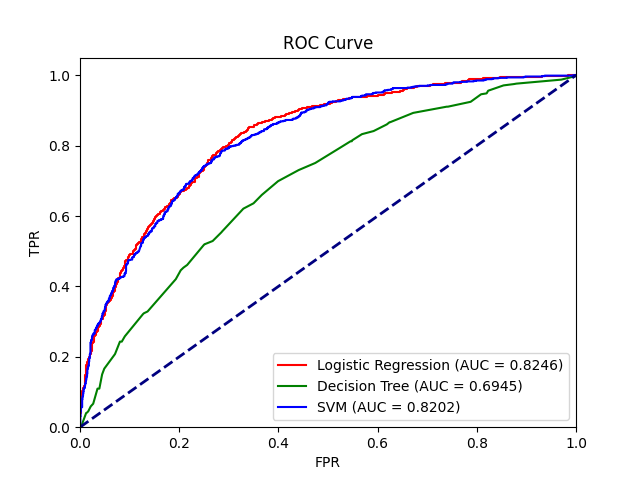
\includegraphics[width=0.9\textwidth]{Figure_1.png}\\
\caption{ROCs of test set}
\label{fig:roc}
\end{figure}
\end{solution}



\end{document}